\documentclass[a4paper,11pt]{article}
\usepackage{array}
\usepackage{tabularx}
\usepackage{booktabs}
\usepackage{graphicx}
\newcommand{\ra}[1]{\renewcommand{\arraystretch}{#1}}
% define the title
\author{ButterFree}
\title{Calendar System}
\begin{document}
% generates the title
\maketitle
% insert the table of contents
\tableofcontents
\newpage
\section{Vision}
Our vision for the Calendar System is to create an easy to use multiuser
scheldule for organizing meetings. We realise that multiple simulair services
already exist. What we want to do, is create a bridge between calendar systems. We want people, who use differnt calendar applications, to plan together.
\newpage

\section{Use cases}
\begin{table*}[ht]\centering
  \ra{1.3}
  \begin{tabularx}{\textwidth}{@{}rXXl@{}}\toprule
    \textbf{ID} & \textbf{Description} & \textbf{Notes} & \textbf{Priority} \\\hline
    1 & The user creates an appointment with another user.             & The
    target can either be in our calendar system or in another iCal compatible
    system. & High \\\hline
    2 & The user accepts an invite to an appointment with another user & Same
    as above
    & High \\
    \bottomrule
  \end{tabularx}
  \caption{Our use cases}
  \label{usecases}\centering% 
\end{table*}
\subsection{Use case 1}
The user wish to create an appointment with another user. The user must first create the appointment in his own calendar system. He then selects the event on our website, and chooses "Invite Attendee". A list of contacts are shown, and the user can select on ore more contacts he wants to invite. The user can add a text to the invitation. The people invited will be notified. The user will receive notification when each invited attendee accepts or declines.
\subsection{Use case 2}
The user has gotten an invitation to an appointment with another user, and he wants to reply.
The user logs on to our website, and finds the invitation in his notifications. The user can press either 'Accept' or 'Decline'. The user can add a text to his reply.
\section{Use Cases UML Diagram}
\begin{figure}[h!]
  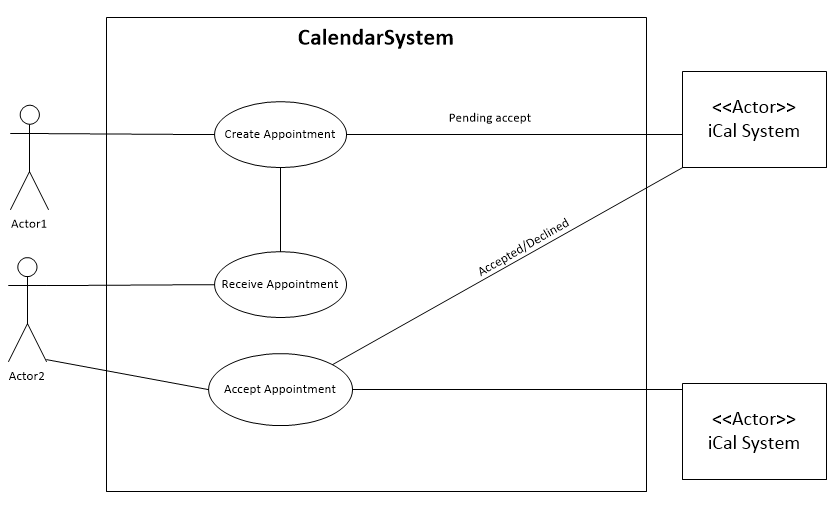
\includegraphics[width=\textwidth,natwidth=839,natheight=508]{illustrations/UseCaseUML.png}
  \caption{The UML diagram for our use cases}
\end{figure}
\newpage

\section{Glossary}
\begin{table*}[ht]\centering
  \ra{1.3}
  \begin{tabularx}{\textwidth}{@{}rX@{}}
    \toprule
    \textbf{Word} & \textbf{Description} \\\hline
    Appointment & An appointment with the data that can be stored in the iCal format \\\hline
    iCal 		& See iCalendar \\\hline
    iCalendar	& iCalendar is a computer file format which allows Internet users to send meeting requests and tasks to other Internet users \\\hline
    Share       & Send an appointment to another user via the iCal format \\\hline
    User        & A user of an iCal compatible system. When several users are mentioned the first one is the user of our system\\
    \bottomrule
  \end{tabularx}
  \caption{Our glossary explaining the terms we use}
  \label{glossary}\centering
\end{table*}
\newpage

\section{Supplementary Requirements}
In this section we will cover any supplementary requirements.
\subsection{Functionality}
\textit{No addition requirements.}
\subsection{Usability}
\textit{No addition requirements.}
\subsection{Reliability}
\begin{itemize}
  \item Our system must be available to our users at least 90\% of the time
\end{itemize}
\subsection{Performance}
\begin{itemize}
  \item Our system must respond in less than 1 sec in 90\% of the cases.
    (External system are out of our control, and this time is therefore
    subtracted)
\end{itemize}
\subsection{Supportability}
\begin{itemize}
  \item Compatible with all iCal-systems.
\end{itemize}
\newpage

\section{Domain Model}
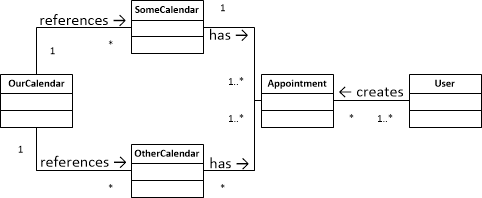
\includegraphics[width=\textwidth,natwidth=482,natheight=198]{illustrations/DomainModel.png}

\section{System Sequence Diagram}
\begin{figure}[h!]
  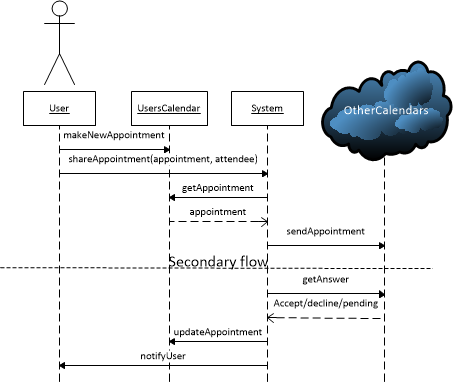
\includegraphics[width=\textwidth,natwidth=453,natheight=382]{illustrations/SSD.png}
  \caption{The sequence diagram for our system}
\end{figure}
\newpage

\end{document}
